\chapter{Objetivos e hipótesis de trabajo}
\label{cap:Objetivo}


\section{Objetivo Principal}
El objetivo principal a abordar será la construcción de un simulador para la predicción de la \textbf{distribución óptima} de energía entre \textbf{elementos generadores} (placas solares, energía almacenada en las baterías de almacenaje, o suministro de la red eléctrica) y \textbf{elementos consumidores} (clientes particulares, venta a la red eléctrica, almacenaje, etc) teniendo en cuenta que toda la energía generada debe ser consumida de una u otra forma.
Este problema podría ser modelado como un problema de satisfacción de restricciones (PSR).
Un problema de satisfacción de restricciones~\cite{Russ06} está caracterizado por:
\begin{itemize}
	\item Un conjunto de variables, donde cada variable dispone de un dominio de valores que puede tomar.
	\item Un conjunto de restricciones, que permite conocer las posibles combinaciones de las variables.
	\item La solución al PSR será la asignación de valores a las variables de forma que se satisfacen las restricciones.
\end{itemize} 
Cómo se puede observar en la Figura 2, la funcionalidad del sistema sería la de modelar cada una de las salidas (cantidad de energía a la baterías, Cbat; cantidad de energía al hogar, Chogar; y cantidad de energía a la red, Cred), en función del valor de cada una de las entradas (potencia suministrada de las placas fotovoltaicas, Pfv; potencia suministrada de la red, Pred; y potencia suministrada de las baterías, Pbat), que representan el conjunto de variables del problema de satisfacción de restricciones. 

\begin{figure}[!h]
	\centering
	\includegraphics[width=9cm]{figs/Esquema.png}
	\caption{Esquema del sistema}
\end{figure}

\section{Objetivos Parciales}
A lo largo del trabajo habrá que satisfacer una serie de subobjetivos necesarios para lograr el objetivo principal tales como:
\begin{enumerate}
	\item \textbf{Identificación y adquisición de los datos y variables que definen el sistema:}
	Se estudiarán las entradas del sistema y el grado de importancia que tiene cada una en cada situación. La información meteorológica de las próximas 24 horas será obtenida utilizando una API oficial de AEMET~\cite{Aemet}, y los datos del mercado eléctrico serán obtenidos utilizando la API oficial e-sios de Red Eléctrica de España S.A.~\cite{Esios} 
	
	\item \textbf{Establecer las relaciones y restricciones propias del consumo eléctrico:}
	Las variables obtenidas en el objetivo anterior estarán sujetas a unas restricciones que nos permitirán conocer las combinaciones posibles de valores, teniendo en cuenta que toda la energía generada debe ser consumida de alguna forma, ya sea por medio de venta a clientes, venta a la red eléctrica, o cargada en baterías de almacenaje.
	
	\item \textbf{Añadir una IA para la generación optimizada de energía y dar lugar a una planificación:}
	Una vez obtenidos los datos y variables del problema y conociendo el grado de implicación de los mismos, se creará un modelo del sistema con una planificación temporal de 24 horas. Esto se podrá llevar a cabo incorporando inteligencia artificial, mediante \textbf{redes LSTM} (Long Short Term Memory)~\cite{Brow07}.
	Las redes LSTM son empleadas en problemas de predicción de secuencia, diferentes a otros problemas de aprendizaje supervisado. En una secuencia existe un orden que debe preservarse a la hora de entrenar el modelo y realizar predicciones, como ocurrirá en nuestro caso. Implementar un problema de este tipo con una red neuronal clásica (perceptrón multicapa) es posible pero tiene algunas limitaciones, ya que carece de una estructura temporal y sus entradas son de tamaño fijo. Por su parte, las redes LSTM cuentan con una formulación única que permite evitar problemas que impiden el entrenamiento obteniendo muy buenos resultados. Es por esto que se ha decidido implementar el modelo de predicción a partir de ellas.
	\item \textbf{Simular la planificación:}
	Se llevará a cabo la simulación de la planificación realizando un seguimiento y una comprobación de la desviación que se puede haber producido con respecto a los datos reales. A partir de lo deducido en la simulación anterior, se tomará la decisión de ajustar o no el modelo para futuras predicciones.
\end{enumerate}

Introduce y motiva la problemática (i.e.\emph{\ ¿cuál es el problema que se plantea y porqué es interesante su resolución?})

Debe concretar y exponer detalladamente el problema a resolver, el entorno de trabajo, la situación y qué se pretende obtener. También puede contemplar las limitaciones y condicionantes a considerar para la resolución del problema (lenguaje de construcción, equipo físico, equipo lógico de base o de apoyo, etc.). Si se considera necesario, esta sección puede titularse \emph{Objetivos del TFG e hipótesis de trabajo}. En este caso, se añadirán las hipótesis de trabajo que el alumno pretende demostrar con su TFG.

Una de las tareas más complicadas al proponer un TFG es plantear su \textsf{Objetivo}. La dificultad deriva de la falta de consenso respecto de lo que se entiende por \emph{objetivo} de un trabajo de esta naturaleza. En primer lugar se debe distinguir entre dos tipos de objetivo:

\begin{enumerate}
	\item La \emph{finalidad específica} del TFG que se plantea para resolver una problemática concreta aplicando los métodos y herramientas adquiridos durante la formación académica. Por ejemplo, \emph{<<Desarrollo de una aplicación software para gestionar reservas hoteleras \emph{on-line}>>}.
	
	\item El \emph{propósito académico} que la realización de un TFG tiene en la formación de un graduado. Por ejemplo, la \emph{adquisición de competencias específicas de la especialización} cursada.
\end{enumerate}

En el ámbito de la memoria del TFG se tiene que definir el primer tipo de objetivo, mientras que el segundo tipo de objetivo es el que se añade al elaborar la propuesta de un TFG presentada ante un comité para su aprobación. Este segundo tipo de objetivo no debe incluirse en el apartado correspondiente de la memoria y en todo caso puede valorarse su satisfacción en la sección de resultados y conclusiones.

Un objetivo bien planteado para el TFG debe estar determinado en términos del \emph{<<producto final>>} esperado que resuelve un problema específico. Es por tanto un sustantivo que debería ser \emph{concreto} y \emph{medible}. El \textsf{Objetivo} planteado puede pertenecer una de las categorías que se indica a continuación:
\begin{itemize}
	\item \emph{Diseño y desarrollo de <<artefactos>>} (habitual en las ingenierías),
	\item \emph{Estudio} que ofrece información novedosa sobre un tema (usual en las ramas de ciencias y humanidades), y
	\item \emph{Validación de una hipótesis} de partida (propio de los trabajos científicos y menos habitual en el caso de los TFG).
\end{itemize}

Estas categorías no son excluyentes, de modo que es posible plantear un trabajo cuyo objetivo sea el diseño y desarrollo de un <<artefacto>> y éste implique un estudio previo o la validación de alguna hipótesis para guiar el proceso. En este caso y cuando el objetivo sea lo suficientemente amplio puede ser conveniente su descomposición en elementos más simples hablando de \emph{subobjetivos}. Por ejemplo, un programa informático puede descomponerse en módulos o requerir un estudio previo para plantear un nuevo algoritmo que será preciso validar. 

La descomposición de un objetivo principal en subobjetivos u objetivos secundarios debería ser natural (no forzada), bien justificada y sólo pertinente en los TFG de gran amplitud.

Junto con la definición del objetivo del TFG se puede especificar los \emph{requisitos} que debe satisfacer la solución aportada. Estos requisitos especifican \emph{características} que debe poseer la solución y \emph{restricciones} que acotan su alcance. En el caso de TFG cuyo objetivo es el desarrollo de un <<artefacto>> los requisitos pueden ser \emph{funcionales} y \emph{no funcionales}.

Al redactar el objetivo de un TFG se debe evitar confundir los medios con el fin. Así es habitual encontrarse con objetivos definidos en términos de las \emph{acciones} (verbos) o \emph{tareas} que será preciso realizar para llegar al verdadero objetivo. Sin embargo, a la hora de planificar el desarrollo del trabajo si es apropiado descomponer todo el trabajo en \emph{hitos} y estos en \emph{tareas} para facilitar dicha \emph{planificación}.

%El motivo de tal confusión deriva de <<mezclar>> la definición de la finalidad específica del TFG con el propósito académico del mismo.

La categoría del objetivo planteado justifica modificaciones en la organización genérica de la memoria del TFG. Así en el caso de estudios y validación de hipótesis el apartado de resultados y conclusiones debería incluir los resultados de experimentación y los comentarios de cómo dichos resultados validan o refutan la hipótesis planteada.

